\chapter{Related Work}\label{ch:Related Work}

\subsection{Inverse problem}
The process of reconstructing 3D structures from TEM tilt series is a challenging and ill-posed inverse problem. In this process, a volume is reconstructed from finite and noisy 2D projections by inverting the advanced visualization model, which projects the 3D structure to the observed dimensions \cite{Lin2020}. This allows the volume to be recovered from the 2D projections. Traditional algorithms, such as back projection, are incapable of fully addressing the ill-posed Ness of the problem because of its structural dimension.

\vspace{20pt}

\begin{figure}[thbp]
    \centering
    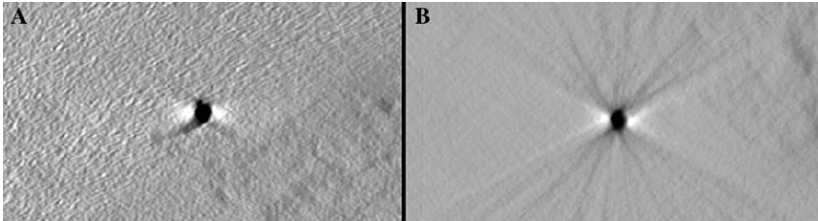
\includegraphics[width=.9\textwidth]{img/Inverse Problem.png}
    \caption{Comparative Reconstruction of a 10 nm Diameter Gold Particle: (A) Using Linear Backprojection in IMOD Software, showing deviation from spherical shape. (B) Using Curvilinear Backprojection in TxBR, accurately representing a spherical particle \cite{Lawrence2006}.  }\label{fig: Inverse problem comparative reconstruction}
\end{figure}

\vspace{10pt}


Regularized iterative reconstruction approaches have been created as a means of overcoming restrictions that are unique to analytical methods \cite{Widmer2013}. These strategies integrate past knowledge in order to limit the space available for solutions. Total variation (TV), a technique for regularization that creates reconstructions with smoothed intensity variations while keeping edges \cite{Widmer2013}, is a technique that is extensively utilized. Compressive sensing is an additional method that makes use of sparsity in transform domains such as gradients or wavelets \cite{Sorzano2004}. In addition, patch-based sparse coding methods have been utilized in order to discover an exhaustive collection of local basis functions for the purpose of denoising \cite{Zhang2017}. However, when the amount of data grows larger, these methods experience a rise in the computational burdens they must bear, and choosing the appropriate regularization parameters becomes a process that is not easy to do.

\vspace{10pt}


The inclusion of a missing wedge, which results from the limited tilt range, low signal-to-noise ratios, and high volumes of the 3D data \cite{Fernandez2012}, further complicates the TEM reconstruction process. More resilient regularization techniques that are specially tailored to the imaging physics of TEM are required to get beyond these challenges. Estimating the point spread function of the microscope using model-based methods has been suggested as a way to invert the blurring effects of the instrument \cite{Fernandez2012}. 

\vspace{10pt}

To enhance the quality of the reconstruction, one method that does so by capitalizing on the self-similarity that exists between blocks is known as non-local means filtering \cite{Lawrence2006}. In recent years, learning-based algorithms, such as dictionary learning and deep convolutional networks \cite{Zhang2017}, have demonstrated promising results as post-processing filters or end-to-end reconstruction methods.
\vspace{15pt}

In the realm of TEM reconstruction, the development of more recent deep 3D representations, such as generative adversarial networks and neural radiance/volumetric fields \cite{Moawad2020}, has made room for the introduction of new prospects. These methods involve training networks to map real noisy TEM projections to cleaner target volumes, which enables the networks to implicitly encode appropriate priors for accurate reconstruction. However, in order for these methods to work, a substantial amount of training data that covers the entire spectrum of viewing angles is required. Despite these developments, modeling the process of TEM image creation and adapting regularization limitations are still open difficulties that need to be addressed. There is a possibility that hybrid approaches, which combine model-based reconstruction with learned regularization techniques, could provide a more resilient solution.

\vspace{10pt}


\clearpage
\subsection{Atomic Resolution}

Atomic-resolution transmission electron microscopy (TEM) has emerged as a revolutionary technique for materials characterization by directly imaging individual atoms \cite{Kawahara2022}. Modern TEMs use aberration correctors and monochromators that eliminate chromatic blurring and lens flaws to achieve sub-angstrom resolution \cite{Krivanek2010}. Advanced detectors and highly stable devices have created new opportunities for quantitative analysis \cite{Wastl2013}.

\vspace{5pt}

\begin{figure}[thbp]
    \centering
    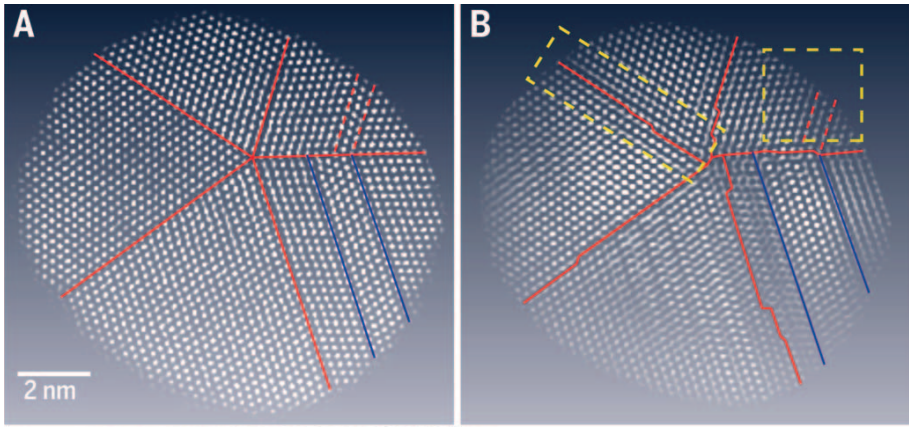
\includegraphics[width=.8\textwidth]{img/Atomic Resolution.png}
    \caption{Atomic Resolution 3D Imaging of Platinum Nanoparticle: (A) STEM image showing flat twin boundaries. (B) AET reconstruction reveals atomic steps at twin boundaries, with a grain boundary and stacking fault \cite{Miao2016}.}\label{fig: Atomic Resolution comparative reconstruction}
\end{figure}

On atomic structures, many imaging techniques offer complimentary information. Atomic number contrast images are created through high angle annular dark field (HAADF) imaging, where the intensity scales with Z2 \cite{Miao2016}. Elemental distributions are mapped by atomically resolved energy dispersive X-ray (EDX) spectroscopy. High resolution TEM can image light elements and even depict atom columns. For high precision data, scanning TEM (STEM) raster scans a focused probe \cite{MacLaren2014}.High beam currents within a tiny probe are necessary for atomically detailed imaging, though. As a result, the electron dosages exceed what many materials can tolerate in terms of radiation \cite{Muller2009}. The fundamentally probabilistic electron-sample interactions thus mask important atomic organization details with quantum noise \cite{Linck2016}. Robust denoising techniques designed for TEM are necessary to obtain quantitative data.
\vspace{10pt}

Through statistical post-processing, techniques like multi-frame averaging \cite{MacLaren2014} and principal component analysis enhance signal-to-noise. Sparse regularization techniques take advantage of structural redundancy to reduce noise. Compact representations for denoising are discovered through dictionary learning \cite{Miao2016}. Convolutional neural networks have most recently demonstrated the ability to learn potent priors from atomistic image simulations \cite{Miao2016}. In general, the developments that have been made in aberration corrected TEM have effectively actualized single-atom sensitivity and precision \cite{Linck2016}. Researchers now have capabilities never before seen to unearth new insights through quantitative atomic-scale characterization. These skills are made possible with the assistance of specific denoising techniques, which help researchers overcome resolution restrictions imposed by noise.



\clearpage
\subsection{Noise Modeling}
Accurately modeling and characterizing noise is critical for developing effective reconstruction and denoising methods for transmission electron microscopy (TEM) images. Multiple studies have investigated the noise properties and sources in TEM.
\begin{itemize}
  \item \textbf{Shot Noise}
  
      One of the primary sources of noise is shot noise stemming from the quantum nature of electrons and the stochastic process of electron-sample interaction. Reconstruction and denoising techniques for transmission electron microscopy (TEM) images require precise noise characterization and modeling. The sources and characteristics of noise in TEM have been the subject of numerous investigations \cite{Ishizuka1977}\cite{Nellist1999}. The number of electrons scattered from each part of the specimen fluctuates, leading to signal-dependent shot noise. Robust statistical distributions capture this behavior.
  \item \textbf{Detector Noise}
  
      TEM detectors also introduce additional noise from readout electronics and amplification \cite{Barthel2010}. On CCD cameras, dark current shot noise and readout noise are present. Scintillator-photomultiplier detectors show signal-dependent Poisson noise characteristics \cite{Ruskin2013}. Accurate detector models enable simulation of cumulative noise.
  \item \textbf{Beam Current Noise}
  
      Fluctuations in beam current and brightness over time also contribute noise in TEM imaging \cite{Faruqi2011}. Monitoring beam current during acquisition allows normalization to reduce this noise \cite{Faruqi2011} \cite{Sang2014}. But residual fluctuations persist and should be incorporated into models.
  \item \textbf{Noise Texture}
  
      The microscope point spread function and optical transfer function modulate the texture of noise in the images. Accurately modeling these effects based on system parameters enables generating realistic synthetic noise for training machine learning models \cite{Ishizuka1980}.
  \item \textbf{Multiresolution Modeling}
  
       Noise also exhibits signal-dependency and non-stationarity over spatial frequencies \cite{Falsini2023}\cite{Jones2015}. Variance stabilization using multiresolution transforms has been proposed to normalize noise over different scales \cite{Boulanger2007}.
  
\end{itemize}

Overall, rigorous characterization and modeling of the multiple noise sources and their interactions is key to developing optimized TEM reconstruction and restoration techniques. Both model-based and learning-based methods benefit from accurate noise models matched to real TEM imaging.

\clearpage

\subsection{3D Convolutional Neural Networks}
3D Convolutional Neural Networks (CNNs) are a powerful tool that leverage the unique characteristics of 3D context and convolution operations to perform a wide array of tasks such as segmentation, classification, and reconstruction of volumetric data. Among the various architectures available, the 3D U-Net has demonstrated exceptional performance, particularly in the field of medical image analysis, by utilizing encoder-decoder convolutions \cite{cicek2016}.


\vspace{10pt}


\begin{figure}[thbp]
    \centering
    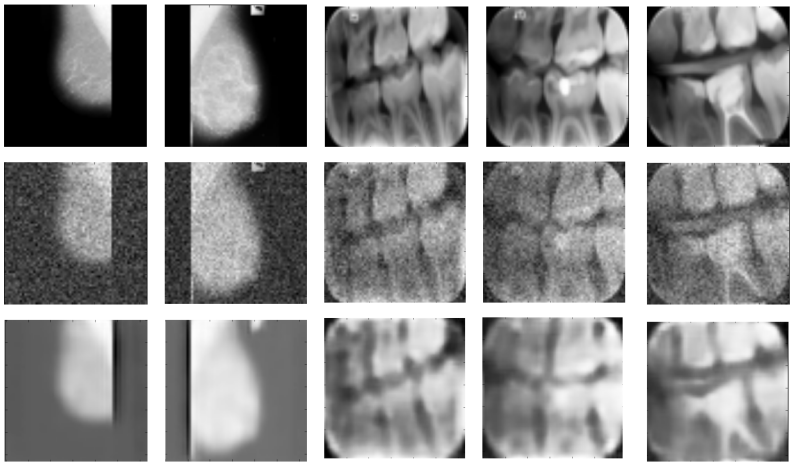
\includegraphics[width=.6\textwidth]{img/3D Convolutional Neural Networks.png}
    \caption{First row - Original real images, Second row - Noisier versions, Third row - Images after denoising with CNN DAE \cite{cicek2016}.}\label{fig: Medical Image of 3D CNN Denoising}
\end{figure}

One of the key benefits of 3D CNNs is their ability to act as data-driven filters that can denoise Transmission Electron Microscopy (TEM) volumes, thus enhancing the interpretability of these volumes. For instance, 3D convolutional autoencoders that have been specifically trained to reconstruct TEM data can effectively serve as noise suppression filters \cite{Gondara}. The process of applying 3D CNN denoising before proceeding with coordinate-based Multilayer Perceptron (MLP) modeling may significantly help condition the data, making it more suitable for further analysis.
\vspace{10pt}

Combining Volumetric CNNs and Coordinate MLPs for Improved Performance
In recent years, hybrid methods that merge the functionalities of volumetric CNNs and coordinate MLPs have been developed, demonstrating potential for improved reconstruction outcomes by leveraging their complementary strengths \cite{Moawad2020} \cite{Zhang2017}. In such a hybrid approach, volumetric CNN encoders first aggregate global context from the 3D input data. Subsequently, coordinate-based MLP decoders model local relationships at each individual location.
\vspace{10pt}

This unique combination enables the joint learning of multi-scale representations, in which the CNN provides top-down semantic guidance, while the MLP preserves the bottom-up spatial details. In the context of TEM data, this dual approach could effectively capture both anatomical priors and the fine structural variations that are typically present. The global-local modeling provided by this combination may enable accurate reconstruction from sparse, noisy tilt series projections, thereby potentially revolutionizing the way we handle and interpret such data.


\clearpage
\subsection{Denoising}

Reducing noise in transmission electron microscopy (TEM) images is critical for enabling accurate reconstruction and analysis. However, the low electron doses used in TEM result in extremely low signal-to-noise ratios. Conventional linear filters like Gaussian smoothing remove noise at the expense of blurred structural details. More advanced model-based methods are not robust to non-Gaussian noise encountered in TEM.
\vspace{10pt}

A variety of denoising methods have been developed for TEM images, including median filtering, Wiener filtering, wavelet transform-based denoising, and deep learning-based denoising \cite{6168375}. Median filtering is a simple and efficient method, but it can blur image edges. Wiener filtering can preserve image edges, but it can be computationally expensive. Wavelet transform-based denoising is a good compromise between efficiency and image quality \cite{6168375}. 
\vspace{10pt}

\begin{figure}[thbp]
    \centering
    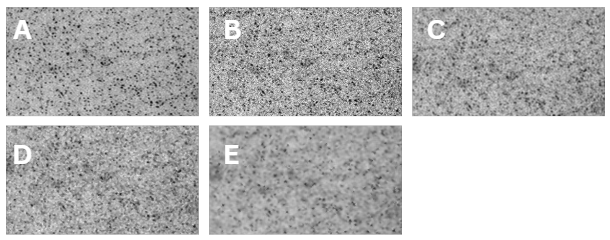
\includegraphics[width=.8\textwidth]{img/Denoising .png}
    \caption{TEM Imaging and Denoising of Cadmium Sulfide Nanoparticles: \textbf{A.} Original Image, \textbf{B.} Image with Gaussian Noise, \textbf{C.} Denoised with Average Filter, \textbf{D.} Denoised with Median Filter, \textbf{E.} Denoised with Weiner Filter \cite{6168375}.
}\label{fig: Filtering Method on Denoising}
\end{figure}

For denoising, sparse coding techniques take advantage of priors in the image such as non-local self-similarity and local sparsity. Sparsifying transforms are used by methods such as K-SVD  \cite{Elad2006} and BM3D to group comparable patches and filter noise. Computational expenses do not scale well with the magnitude of medical images, despite being effective. There are difficulties in choosing regularization parameters optimally.
\vspace{10pt}

Deep learning approaches have recently shown great promise for image denoising by learning data-driven filters \cite{Zhang2017}. Convolutional networks trained as discriminators between clean and noisy image patches can implicitly model complex image priors. Recurrent inference further boosts quality\cite{Zhang2017}. Autoencoder architectures directly optimize reconstruction loss \cite{Zhang2017}. Multi-image network training leverages complementary information across tilt series.
\vspace{10pt}

Applying and tailoring deep denoisers to 3D TEM data could significantly enhance reconstruction quality from noisy tilt projections. The high capacity of deep networks may better capture noise characteristics compared to hand-crafted models. Overall, learned denoising provides new opportunities to overcome resolution limits imposed by noise in TEM imaging.

